\documentclass[a4paper,10pt]{article}
\usepackage[utf8x]{inputenc}
\usepackage{verbatim}
\usepackage{graphicx}
\usepackage{enumerate}

%opening
\title{Lab 6}
\author{William Richard}

\begin{document}

\maketitle

\section{Types of Files}
\subsection{Regular}
  \begin{center}
  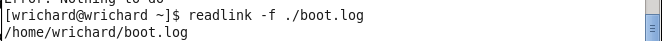
\includegraphics[width=\linewidth]{./regular.png}
  \end{center}

\subsection{Directory}
  \begin{center}
  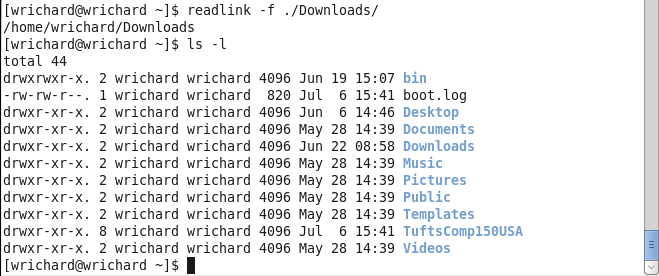
\includegraphics[width=\linewidth]{./directory.png}
  \end{center}

\subsection{Soft Link}
  \begin{center}
  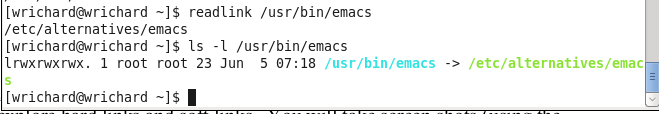
\includegraphics[width=\linewidth]{./link.png}
  \end{center}

\subsection{Character}
  \begin{center}
  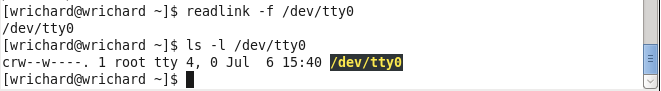
\includegraphics[width=\linewidth]{./character.png}
  \end{center}

\subsection{Block}
  \begin{center}
  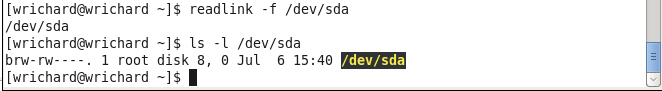
\includegraphics[width=\linewidth]{./block.png}
  \end{center}

\subsection{Named Pipe}
  \begin{center}
  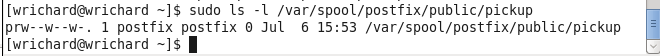
\includegraphics[width=\linewidth]{./pipe.png}
  \end{center}

\subsection{Socket}
  \begin{center}
  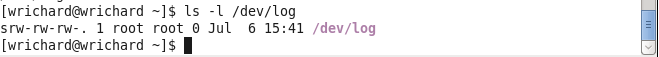
\includegraphics[width=\linewidth]{./socket.png}
  \end{center}

\section{Links}
\subsection{Hard Links}
\subsubsection{Just hlink}
  \begin{center}
  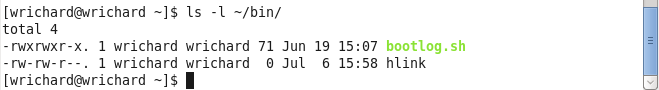
\includegraphics[width=\linewidth]{./hlink1.png}
  \end{center}

\subsubsection{hlink2}
  \begin{center}
  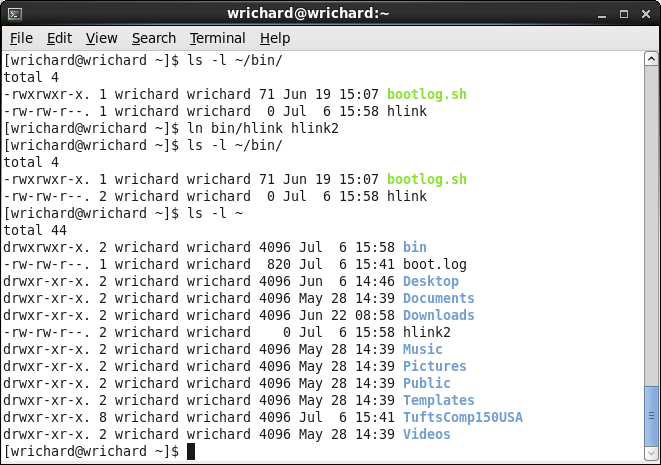
\includegraphics[width=\linewidth]{./hlink2.png}
  \end{center}

\subsubsection{hlink3}
  \begin{center}
  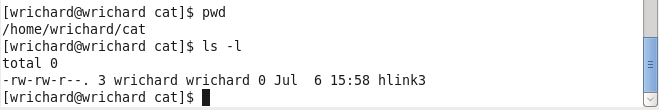
\includegraphics[width=\linewidth]{./hlink3.png}
  \end{center}

\subsubsection{inode values}
  \begin{center}
  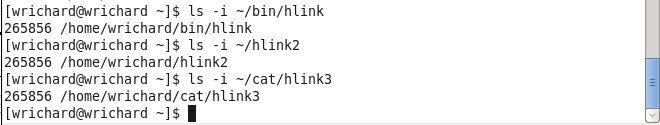
\includegraphics[width=\linewidth]{./hlink_inode.png}
  \end{center}

\subsubsection{Only hlink2 remaining}
  \begin{center}
  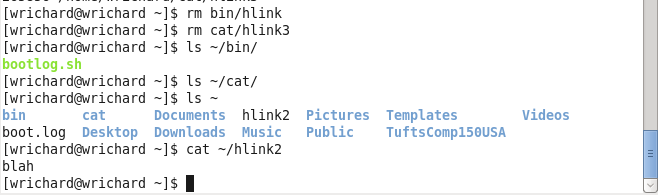
\includegraphics[width=\linewidth]{./rmhlink.png}
  \end{center}

\subsection{Soft Link}
\subsubsection{Original slinks}
  \begin{center}
  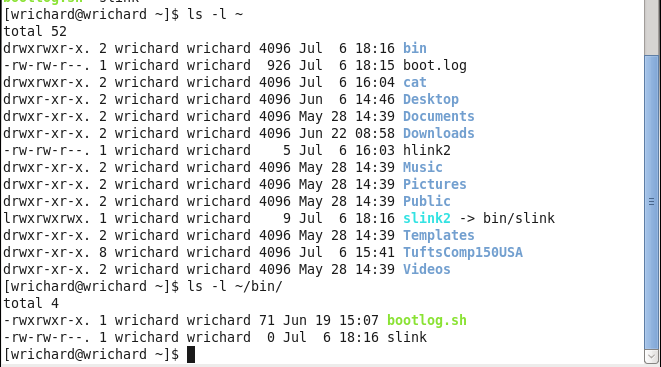
\includegraphics[width=\linewidth]{./slink_empty.png}
  \end{center}
The hard links all had the same size, because they were the same file. The soft links have different sizes, because (as you said) slink2 only points to the location of slink, rather than being the ``same'' object.
\subsubsection{slink contents and inode values}
  \begin{center}
  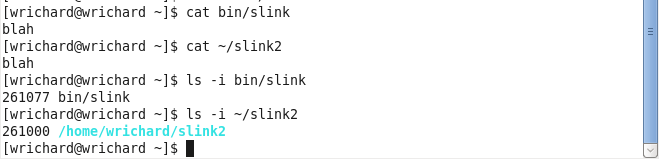
\includegraphics[width=\linewidth]{./slink_inode.png}
  \end{center}

\subsubsection{Broken slink2}
  \begin{center}
  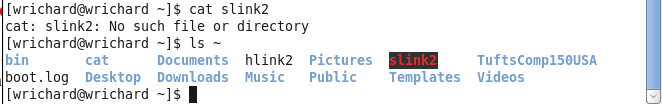
\includegraphics[width=\linewidth]{./broken_slink2.png}
  \end{center}

\subsubsection{New slink}
  \begin{center}
  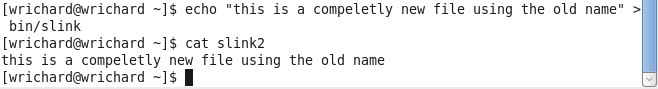
\includegraphics[width=\linewidth]{./new_slink.png}
  \end{center}

\section{chmod}
\begin{enumerate}
 \item chmod 0760 $<$file$>$

chmod -r 0760 network.analysis/
  \item chmod -r u+a,g+rw network.analysis/
  \item 
\end{enumerate}

\section{Mounting Filesystem}
\subsection{dmesg for sdb}
  \begin{center}
  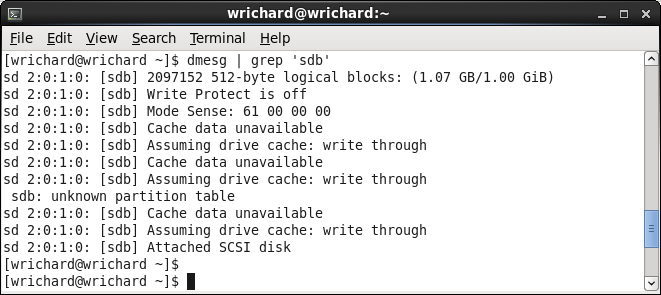
\includegraphics[width=\linewidth]{./new_drive_dmesg.png}
  \end{center}

\subsection{fdisk}
  \begin{center}
  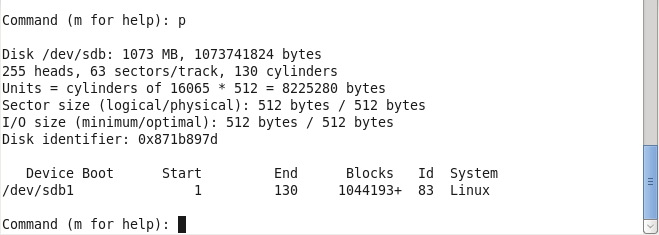
\includegraphics[width=\linewidth]{./fdisk_info.png}
  \end{center}

\subsection{sdb1 mounted df -h}
  \begin{center}
  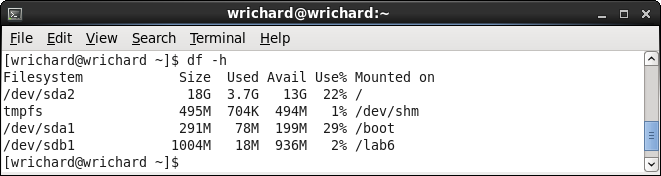
\includegraphics[width=\linewidth]{./sdb1_mounted.png}
  \end{center}

\subsection{ls -l lab6}
  \begin{center}
  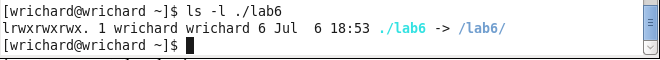
\includegraphics[width=\linewidth]{./lab6_soft_link.png}
  \end{center}

\subsection{/etc/fstab}
  \begin{center}
  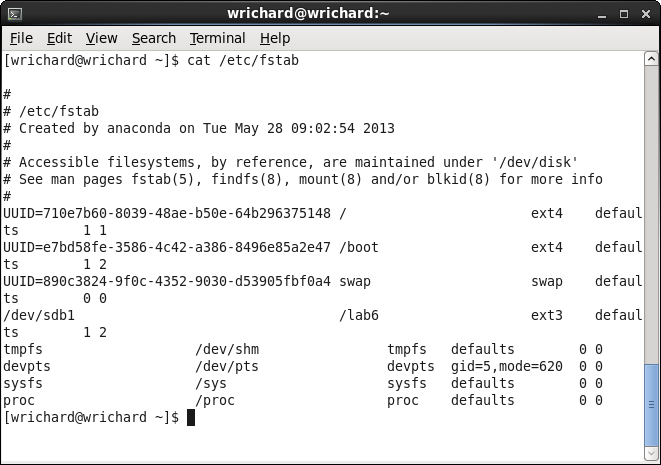
\includegraphics[width=\linewidth]{./fstab.png}
  \end{center}










\end{document}
